% Created 2013-02-12 Tue 11:12
\documentclass[11pt]{article}
\usepackage[utf8]{inputenc}
\usepackage[T1]{fontenc}
\usepackage{fixltx2e}
\usepackage{graphicx}
\usepackage{longtable}
\usepackage{float}
\usepackage{wrapfig}
\usepackage{soul}
\usepackage{textcomp}
\usepackage{marvosym}
\usepackage{wasysym}
\usepackage{latexsym}
\usepackage{amssymb}
\usepackage{hyperref}
\tolerance=1000
\providecommand{\alert}[1]{\textbf{#1}}

\title{Discussion 5}
\author{Stephanie Chan}
\date{\today}
\hypersetup{
  pdfkeywords={},
  pdfsubject={},
  pdfcreator={Emacs Org-mode version 7.9.3e}}

\begin{document}

\maketitle


\section{Problem 18.4}
\label{sec-1}

  Refer to Problem 16.7\\
\textbf{Productivity improvement} An economist ecompiled data on productivity
improvements last year for a sample of firms producing electronic
computing equipment.  the firms were classified according to the
level of their average expenditures for research and development in
the past three years (low, moderate, high).  The results of the study
follow (productivity improvemtn is measured on a scale frome 0 to
100).

\begin{center}
\begin{tabular}{lrrrrrrrrrrrr}
\hline
           &    1  &    2  &     3  &    4  &    5  &    6  &    7  &    8  &    9  &   10  &   11  &   12  \\
\hline
 Low       &  7.6  &  8.2  &   6,8  &  5.8  &  6.9  &  6.6  &  6.3  &  7.7  &  6.0  &       &       &       \\
 Moderate  &  6.7  &  8.1  &   9.4  &  8.6  &  7.8  &  7.7  &  8.9  &  7.9  &  8.3  &  8.7  &  7.1  &  8.4  \\
 High      &  8.5  &  9.7  &  10.1  &  7.8  &  9.6  &  9.5  &       &       &       &       &       &       \\
\hline
\end{tabular}
\end{center}
\subsection{Residual dot plots}
\label{sec-1-1}

Prepare aligned residual dot plots by factor level.  What departures
from ANOVA model can be studied from these plots?  What are your
findings?


\begin{verbatim}
Y1 = c(7.6,8.2,6.8,5.8,6.9,6.6,6.3,7.7,6.0)
Y2 = c(6.7,8.1,9.4,8.6,7.8,7.7,8.9,7.9,8.3,8.7,7.1,8.4)
Y3 = c(8.5,9.7,10.1,7.8,9.6,9.5)

Y1bar = mean(Y1)
Y2bar = mean(Y2)
Y3bar = mean(Y3)

residuals = c(Y1-Y1bar,Y2-Y2bar,Y3-Y3bar)
factors = c(rep(1,9),rep(2,12),rep(3,6))

png("dotplot.png")
plot(residuals,factors)
dev.off()
\end{verbatim}

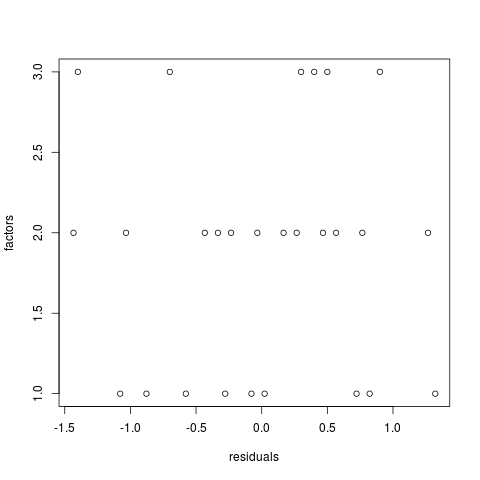
\includegraphics[width=.9\linewidth]{dotplot.png}
\subsection{Normal Probability Plot}
\label{sec-1-2}

Pepare a normal probability plot of the residuals.  Also obtain the
coefficients of correlation betwee the ordered residuals and their
expected values under normality.  Does the normality assumption
appear to be reasonable here?

\begin{verbatim}

png("qqnormplot.png")
qqnorm(residuals)
dev.off()
\end{verbatim}

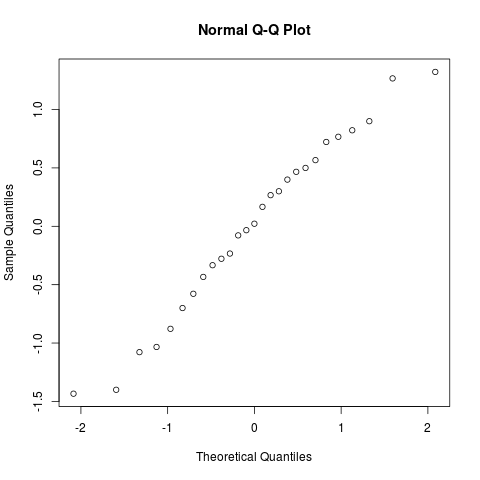
\includegraphics[width=.9\linewidth]{qqnormplot.png}



\begin{verbatim}

# expected residuals
expected = qnorm(ppoints(residuals),0,1)

cor(expected,sort(residuals))
\end{verbatim}
\subsection{Location of Office}
\label{sec-1-3}

The economist wishes to investigate whether location of the firm's
home office is related to productivity improvement.  The home office
locations are as follows (U: U.S.; E: Europe):

\begin{center}
\begin{tabular}{rlllllllllrrr}
\hline
    &  1  &  2  &  3  &  4  &  5  &  6  &  7  &  8  &  9  &  10  &  11  &  12  \\
\hline
 1  &  U  &  E  &  E  &  E  &  E  &  U  &  U  &  U  &  U  &      &      &      \\
 2  &  E  &  E  &  E  &  E  &  U  &  U  &  U  &  U  &  U  &   E  &   E  &   E  \\
 3  &  E  &  U  &  E  &  U  &  U  &  E  &     &     &     &      &      &      \\
\hline
\end{tabular}
\end{center}



Prepare aligned residual dot plots by factor level in which the
location of the home office is identified.  Does it appear that ANOVA
model could be improved by adding location of home office as a second
factor?  Explain.


\begin{verbatim}

loc1 = c('U','E','E','E','E','U','U','U','U')
loc2 = c('E','E','E','E','U','U','U','U','U','E','E','E')
loc3 = c('E','U','E','U','U','E')

locations = c(loc1,loc2,loc3)

Uresiduals = residuals[locations=='U']
Ufactors = factors[locations=='U']
png("USplot.png")
plot(Uresiduals,Ufactors,main="United States Location")
dev.off()

Eresiduals = residuals[locations=='E']
Efactors = factors[locations=='E']
png("Europeanplot.png")
plot(Eresiduals,Efactors,main="European Location")
dev.off()
\end{verbatim}

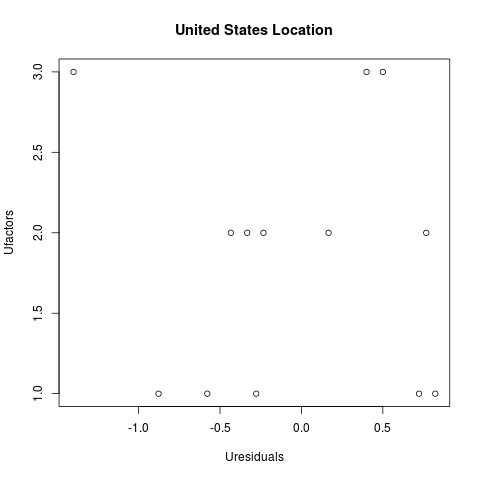
\includegraphics[width=.9\linewidth]{USplot.png}

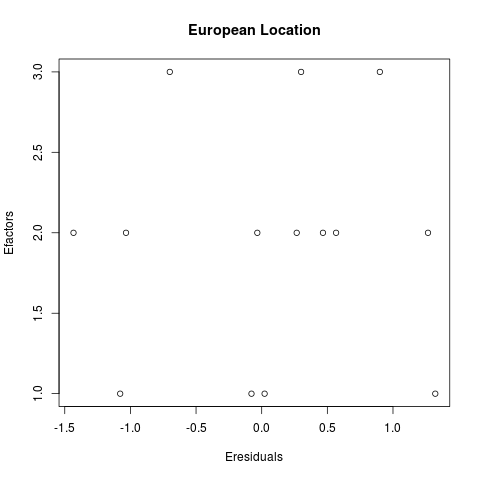
\includegraphics[width=.9\linewidth]{Europeanplot.png}

\end{document}
